\documentclass[11pt]{beamer}
\usetheme{Malmoe}
\usepackage[utf8]{inputenc}
\usepackage[czech]{babel}
\usepackage[T1]{fontenc}
\usepackage{amsmath}
\usepackage{amsfonts}
\usepackage{amssymb}
\usepackage{graphicx}
\usepackage{enumitem}
\usepackage{listings}

\author{Jan Tušil}
\title{První kroky s Frama-C}
%\setbeamercovered{transparent} 
%\setbeamertemplate{navigation symbols}{} 
%\logo{} 
%\institute{} 
\date{16. 3. 2015} 
%\subject{} 


\lstset{
	language=C++,
	basicstyle=\ttfamily\footnotesize,
%	keywordstyle=\color{red}
}

% see http://tex.stackexchange.com/questions/130643/nested-itemize-environment-affects-vertical-spacing-of-parent-itemize-environmen
% redefine default beamer item labels
\setitemize{label=\usebeamerfont*{itemize item}%
	  \usebeamercolor[fg]{itemize item}
	    \usebeamertemplate{itemize item}}

\begin{document}

\begin{frame}
\titlepage
\end{frame}

\begin{frame}
\frametitle{Table of Contents}
\tableofcontents[]
\end{frame}

\section{Úvod}

\begin{frame}{Materiály k prezentaci}
\begin{itemize}
	\item \url{https://github.com/h0nzZik/Frama-C_Examples}
\end{itemize}
\end{frame}

\begin{frame}{Představení}

\begin{figure}
	
\includegraphics[scale=0.3]{frama-c.png}
\end{figure}

\begin{itemize}
	\item Statická analýza C kódu
	\item Založeno na pluginech
	\item Ověřování proti specifikaci (jazyk ACSL)
	\item Možná specifikace: absence běhových chyb
\end{itemize}

\end{frame}

\begin{frame}{Jak získat?}

\end{frame}


\section{Jazyk ACSL}

\begin{frame}{ACSL - Co je to za jazyk?}
\begin{itemize}
	\item ANSI / ISO C Specification language
	\item V komentářích C kódu.
	\item Asserty
	\item Invarianty
	\item Funkční kontrakty (DbC)
	\item http://frama-c.com/acsl.html
\end{itemize}
\end{frame}

\begin{frame}{ACSL - vyjadřovací schopnosti}
\begin{itemize}
	\item C operátory a datové typy
	\item Matematické datové typy
	\item Prvořádová logika (s rozšířeními)
\end{itemize}
\end{frame}


\subsection{Jazykové konstrukce}

\defverbatim[colored]\lstBasicAssert{
\begin{lstlisting}[language=C++]
int x = 17;
/*@ assert x > 5 */
\end{lstlisting}
}

\begin{frame}{Asserty}
\lstBasicAssert
\begin{itemize}
	\item Základní specifikační jednotka
	\item Tvrzení o stavu programu v daném bodě.
	\item (ACSL specifikace zabudována v komentáři)
\end{itemize}
\end{frame}

\defverbatim[colored]\lstQuantifiedAssert{
\begin{lstlisting}
int array[4] = {-15, 3, 17, 104};
/*@
assert \forall integer i, j;
0 <= i <= j < 4 ==> array[i] <= array[j];
*/
\end{lstlisting}
}


\begin{frame}{Kvantifikátory}
\lstQuantifiedAssert
\begin{itemize}
	\item Vázaná proměnná má daný typ
	\item Typ může být uživatelem definovaný
	\item \texttt{integer} označuje (matematické) celé číslo
\end{itemize}
\end{frame}


\defverbatim[colored]\lstPointerValidity{
\begin{lstlisting}
int array[4] = {-15, 3, 17, 104};	
/*@ assert \valid(array + (0..3)); */
\end{lstlisting}
}

% TODO: kod na slajdech by mohl byt zarovnany vzdy stejne

\begin{frame}{Pointery}
\lstPointerValidity
\begin{itemize}
	\item Predikát \textbackslash valid bere množinu termů
	\item \(0..3\) označuje množinu \( \{ 0, 1, 2, 3 \} \)
	\item Význam: výrazy \( \{ array + 0, \ldots , array + 3 \} \) jsou platné ukazatele
	\item Obvyklá pointer aritmetika
\end{itemize}
\end{frame}

\defverbatim[colored]\lstPredicateSorted{
\begin{lstlisting}
/*@
predicate is_sorted ( int *array, integer len ) = 
\forall integer i, j; 0 <= i <= j < len
==> array[i] <= array[j];
*/
\end{lstlisting}
}

\defverbatim[colored]\lstPredicateSortedUsed{
\begin{lstlisting}
/*@ assert is_sorted ( array, 4 ); */
\end{lstlisting}
}

\begin{frame}{Uživatelské predikáty}
\lstPredicateSorted
\begin{itemize}
\item Predikát lze využít později
\end{itemize}
\lstPredicateSortedUsed
\end{frame}

\defverbatim[colored]\lstLoopWithInvariant{
\begin{lstlisting}
int arr[7];
[ ... ]
/*@ loop invariant is_sorted(arr, i) */
for ( int i = 0; i < 7; i++ ) {
	[ ... ]
}
\end{lstlisting}
}

\begin{frame}{Invarianty smyček}
\lstLoopWithInvariant
\end{frame}

\defverbatim[colored]\lstFunctionContract{
\begin{lstlisting}
/*@
requires \valid ( array + (0 .. ( len-1 ) ) );
ensures is_sorted ( array, len );
 */
void sort ( int *array, size_t len);
\end{lstlisting}
}

\begin{frame}{Funkční kontrakty}
\lstFunctionContract
\begin{itemize}
	\item Paradigma "Design by Contract"
\end{itemize}
\end{frame}

\section{Použití Frama-C}

\begin{frame}{Jednoduché použití}
\begin{itemize}
	\item Soubor hello.c je v adresáři 01\_hello
	\item \lstinline[language=bash]{$ frama-c hello.c -val}
	\item Jak ověřit větší projekt z více souborů?
\end{itemize}
\end{frame}


\subsection{Příprava zdrojových kódů}

\begin{frame}{Na co je preprocesor v C?}
\begin{itemize}
	\pause \item Makra a náhrady textu
	\pause \item Vkládání (hlavičkových) souborů
\end{itemize}
\end{frame}

\begin{frame}{Preprocessing ve Frama-C}
\begin{itemize}
	\item Výchozí: \lstinline[language=bash]{gcc -C -E -I}
	%FIXME: 'command se zobrazi cervene, protoze je to jeden z builtinu bashe
	\item Možno předefinovat přepínačem \lstinline[language=bash]{\-cpp-command}
	\item Frama-C umí předzpracovat i anotace (s GCC)
	\item Rozpracovaný projekt je možné uložit a znovu načíst
	\item Viz soubor build.mk
\end{itemize}
\end{frame}


\begin{frame}{Drobnosti}
	\begin{itemize}
		\item RTE plugin generuje anotace pro obvyklé runtime chyby
		\item Kombinace RTE + Value může prokázat absenci runtime chyb
		\item Uložený projekt je možné načíst do programu frama-c-gui
	\end{itemize}
\end{frame}

\subsection{Value plugin}

\begin{frame}{Value plugin - Principy}
	\begin{itemize}
			\item Abstraktní interpretace
			\item Počítá variační domény proměnných
			\item Overaproximace - dokazuje korektnost
	\end{itemize}
\end{frame}

\begin{frame}{Variační domény}
	\begin{itemize}
			\item Množina možných hodnot, které může obsahovat daná proměnná.
			\item Různé způsoby zápisu
			\begin{itemize}
				\item Výčtem \( \{ 2, 12, 22, 32, 42 \} \)
				\item Intervalem \( [2 \ldots 42], 2 \% 10 \)
			\end{itemize}
	\end{itemize}
\end{frame}

\begin{frame}{Ukázka (01\_hello/hello.c) - 1}
	\begin{figure}
		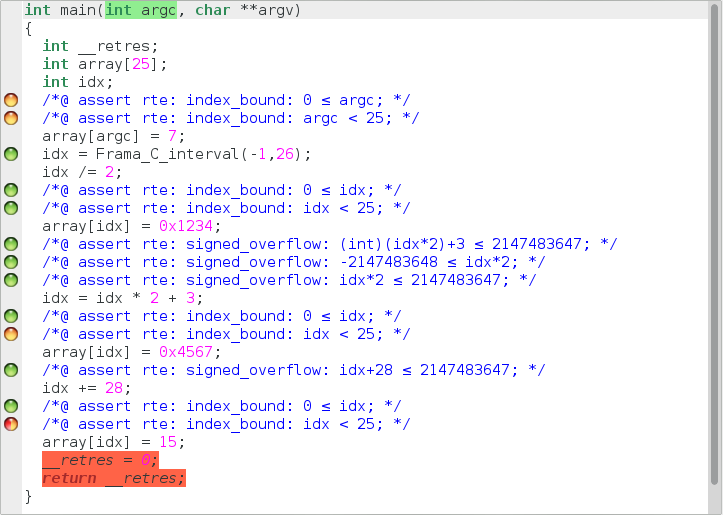
\includegraphics[scale=0.3]{./img/value_01.png}
	\end{figure}
\end{frame}

\defverbatim[colored]\lstFirstValueAnalysis{
\begin{lstlisting}[language=bash]
$ git clone https://github.com/h0nzZik/Frama-C_Examples.git
$ cd Frama-C_Examples/01_hello
$ make
$ frama-c-gui -load project_after_analysis
\end{lstlisting}
}


\begin{frame}{Ukázka (01\_hello/hello.c) - 2}
	\lstFirstValueAnalysis
	\begin{itemize}
			\item Informace vypsané během analýzy jsou k dispozici i v gui
			\item Zajímavé jsou řádky začínající \texttt{hello.c:123:[value]}
	\end{itemize}
\end{frame}

\begin{frame}{Ukázka (01\_hello/hello.c) - 3}
\texttt{hello.c:17:[value] Assertion 'rte,index\_bound' got status unknown.}
	\begin{itemize}
			\item Nelze ověřit, že zápis do pole proběhne v pořádku.
	\end{itemize}
\end{frame}

\subsection{WP plugin}

\section{Omezení}
\subsection{Jazyk}
\begin{frame}{Pouze pro C}
Nikoliv C++
\end{frame}
\subsection{Bugy}


\end{document}
